\documentclass{beamer}
\usetheme[nogauge,amurmapleblue]{Amurmaple}

\usepackage{listings}
\usepackage{xcolor}
\usepackage{booktabs}

\lstset{
  language=Python,
  basicstyle=\ttfamily\small,
  keywordstyle=\color[RGB]{0,112,192}\bfseries,
  stringstyle=\color[RGB]{163,21,21},
  commentstyle=\color[RGB]{106,153,85}\itshape,
  emphstyle=\color[RGB]{78,154,6}\bfseries,
  emph={Model,addVar,addCons,setObjective,optimize,quicksum},
  showstringspaces=false,
  frame=single,
  numbers=none,
  breaklines=true
}

\newcommand{\plugin}[1]{\texttt{#1}}

\title{Let's SCIP it!}
\subtitle{APDIO Workshop: Optimization Software \& Practice}
\author{Jo\~{a}o Dion\'{i}sio}
\date{March 27, 2026}
\titlegraphic{%
  \begin{minipage}{\textwidth}
    \centering
    \raisebox{0.4cm}{
\includegraphics[height=0.5cm]{media/uporto_logo.jpg}}%
    \hspace{1.2cm}%
    
\includegraphics[height=1.2cm]{media/sciplogo.png}%
    \hspace{1.2cm}%
    \raisebox{0.2cm}{
\includegraphics[height=0.7cm]{media/apdio_logo.png}}%
  \end{minipage}%
}

\begin{document}

\begin{frame}
  \maketitle
\end{frame}

% ---------------------------------------------------------
\begin{frame}{What is SCIP?}

\textbf{SCIP} --- \emph{Solving Constraint Integer Programs}

\medskip
\begin{itemize}
  \item Fastest non-commercial solver for mixed-integer programs (MIP/MINLP)
  \item Also handles satisfiability and constraint integer programs
  \item Supports exact arithmetic for MILPs
  \item Open-source under Apache 2.0 license
  \item Under active development for over 20 years (Zuse Institute Berlin)
  \item SCIP alumni work on Gurobi, Xpress, COPT, Hexaly, \ldots
\end{itemize}

\bigskip
\textbf{Interfaces:} C/C++, Python, Julia, Rust, Java, MATLAB

\bigskip
\textbf{File formats:} MPS, LP, CIP, ZIMPL, and more
\end{frame}

% ---------------------------------------------------------
\begin{frame}{Plugin-Based Architecture}

SCIP's real strength: a \textbf{modular plugin system} that lets you
customize every aspect of the solving process.

\medskip
\begin{columns}[T]
\begin{column}{0.45\textwidth}
\textbf{Core framework:}
\begin{itemize}
  \item Branch-and-bound tree
  \item LP solver (SoPlex)
  \item Solution \& cut pools
  \item Conflict analysis
  \item Clique table
\end{itemize}
\end{column}
\begin{column}{0.50\textwidth}
\textbf{Plugins are modular:}
\begin{itemize}
  \item Each type has a defined interface
  \item Called by priority order
  \item Multiple plugins per type
  \item Extend in C, C++, or Python
\end{itemize}
\end{column}
\end{columns}

\bigskip
$\Rightarrow$ Not just a solver --- a \textbf{framework} for building solvers
\end{frame}

% ---------------------------------------------------------
\begin{frame}{Structure of SCIP}
  \begin{center}
    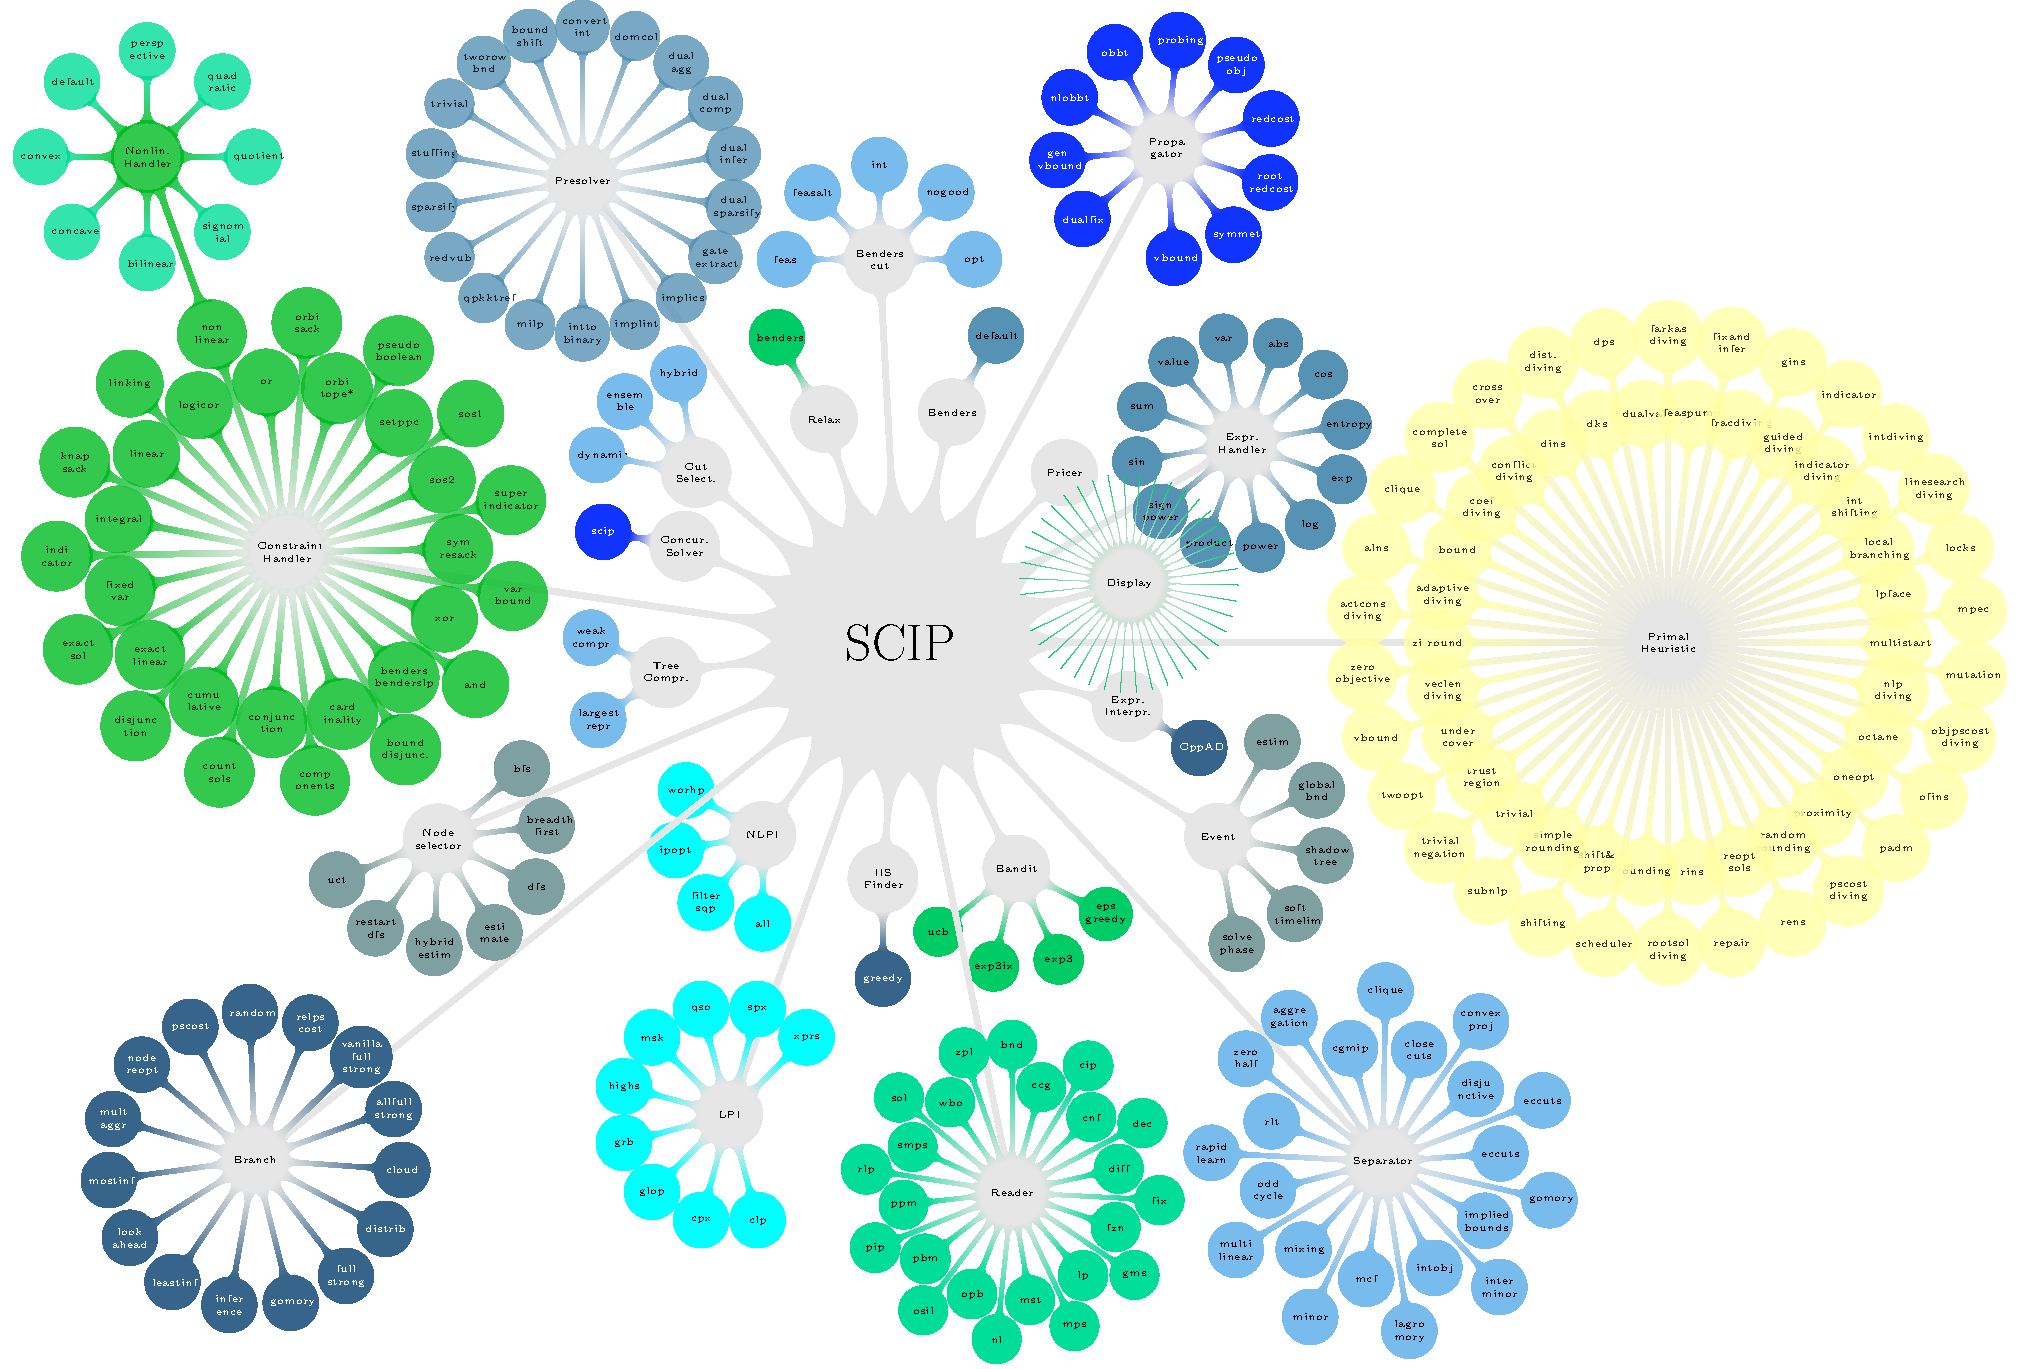
\includegraphics[width=.85\textwidth]{media/scip_structure}
  \end{center}
\end{frame}

% ---------------------------------------------------------
\begin{frame}{Plugin Types}

{\small
\begin{tabular}{@{} l @{\hspace{1em}} l @{\hspace{1em}} l @{}}
\toprule
\textbf{Plugin} & \textbf{Purpose} & \textbf{When} \\
\midrule
\plugin{constraint handler} & feasibility, cuts, propagation & throughout \\
\plugin{separator}          & cutting planes                 & after LP solve \\
\plugin{pricer}             & column generation              & after LP solve \\
\plugin{heuristic}          & find feasible solutions        & configurable \\
\plugin{branching rule}     & split subproblems              & at fractional node \\
\plugin{propagator}         & tighten variable bounds        & at each node \\
\plugin{presolver}          & simplify before solving        & before B\&B \\
\plugin{relaxator}          & custom relaxation bounds       & at each node \\
\plugin{benders}            & Benders decomposition          & throughout \\
\plugin{event handler}      & react to solving events        & on trigger \\
\plugin{node selector}      & pick next subproblem           & after node solved \\
\bottomrule
\end{tabular}
}
\end{frame}

% ---------------------------------------------------------
\begin{frame}{Why SCIP?}

\begin{columns}[T]
\begin{column}{0.48\textwidth}
\textbf{As a black-box solver}
\begin{itemize}
  \item State-of-the-art MIP performance
  \item Nonlinear support (MINLP)
  \item 2000+ tunable parameters
  \item Rich presolving \& heuristics
  \item Reads standard formats
\end{itemize}
\end{column}
\begin{column}{0.48\textwidth}
\textbf{As a framework}
\begin{itemize}
  \item Branch-and-price (pricer)
  \item Row generation (constraint handler)
  \item Custom branching rules
  \item Benders decomposition
  \item Event-driven callbacks
\end{itemize}
\end{column}
\end{columns}

\bigskip
\textbf{You implement the problem-specific logic; SCIP handles the rest.}

\bigskip
SCIP is both a solver and a framework for building custom solvers.
\end{frame}

% ---------------------------------------------------------
\begin{frame}{Today's Workshop}
\begin{enumerate}
  \item \textbf{Part 1 --- Modeling:} build and solve MINLPs in PySCIPOpt
  \item \textbf{Part 2 --- Row Generation:} implement a constraint handler for TSP
  \item \textbf{Part 3 --- Branch-and-Price:} implement a pricer and branching rule for bin packing
\end{enumerate}

\vfill
\begin{center}
  \LARGE \textbf{Let's SCIP it!}
\end{center}
\end{frame}

\end{document}
